\chapter{Outils théoriques du problème à $N$-corps} \label{chap: outils_theoriques}

Ce chapitre présente les outils théoriques essentiels à la compréhension du problème à $N$-corps dans le contexte des méthodes numériques détaillées dans ce mémoire. Nous survolerons la seconde quantification, un formalisme avec lequel on exprime le modèle de Hubbard~\cite{hubbardI, hubbardII, hubbardIII}.

\section{Seconde quantification et modèle de Hubbard} \label{sec: hubbard_model}

\subsection{Modèle de Hubbard}

Grâce au formalisme de la seconde quantification, nous pouvons
exprimer le hamiltonien du modèle de Hubbard~\cite{hubbardI}.
Ce dernier constitue l'un des modèles fondamentaux pour l'étude des systèmes d'électrons fortement corrélés. Il capture la compétition entre l'énergie cinétique, qui favorise la délocalisation des électrons, et l'interaction coulombienne, qui pénalise la double occupation d'un même site. Cette compétition détermine si le système adopte un comportement métallique ou isolant. En utilisant les opérateurs définis précédemment, le hamiltonien s'écrit~:
\begin{align}
    H = -\sum_{i,j,\sigma} t_{ij}c^\dagger_{i\sigma}c_{j\sigma} + U\sum_{i}n_{i\uparrow}n_{i\downarrow}
    -\mu\sum_{i,\sigma}n_{i\sigma},
    \label{eq: hubbard-hamiltonian}
\end{align}
où $c^\dagger_{i\sigma}$ ($c_{i\sigma}$) sont les opérateurs de création (annihilation) d'un électron de spin $\sigma$ au site $i$, $n_{i\sigma}$ est l'opérateur nombre, $t_{ij}$ représente l'amplitude de saut entre les sites $i$ et $j$, $U$ est l'interaction coulombienne sur site et $\mu$ le potentiel chimique. Physiquement, si $t_{ij}\gg U$, les électrons se déplacent librement, comme dans un métal. Inversement, si $U \gg t_{ij}$, ils se localisent pour s'éviter, comme un isolant. La figure~\ref{fig: hubbard-2d} illustre la géométrie du modèle de Hubbard sur réseau carré, montrant les différents paramètres du modèle.
\begin{figure}[h!]
    \centering
    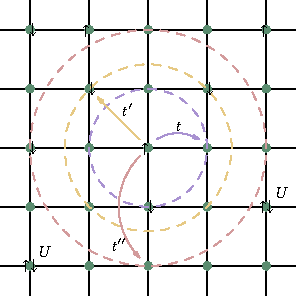
\includegraphics[width=0.45\textwidth]{figs/theorie/2d_lattice.pdf}
    \caption[Modèle de Hubbard sur réseau carré.]{\textbf{Modèle de Hubbard sur réseau carré}. Les cercles de colorés indiquent respectivement les possibilités de sauts aux premiers ($t$), deuxièmes ($t'$) et troisièmes ($t''$) voisins pour un électron de spin $\uparrow$ situé au centre du réseau.}
    \label{fig: hubbard-2d}
\end{figure}

\subsection{Hamiltonien de Hubbard dans la base de Fock}

Pour illustrer concrètement comment le hamiltonien \eqref{eq: hubbard-hamiltonian} s'exprime dans la base de Fock, détaillons d'abord sa dimension. Pour un système de $N$ sites, chaque site peut être dans quatre états soit~: le vide $\ket{0}$, un électron de spin \textit{up} $\ket{\uparrow}$, un électron de spin \textit{down} $\ket{\downarrow}$ ou doublement occupé $\ket{\uparrow\downarrow}$. La dimension totale de l'espace de Fock est donc~:
\begin{align}
    \text{dim}(\mathcal{H}) = 4^N
\end{align}
Cette croissance exponentielle rend la diagonalisation exacte rapidement impossible, comme observé sur le tableau~\ref{tab:hilbert_dimension}.
\begin{table}[h!]
\centering
\begin{tabular}{cc}
\hline
Nombre de sites & $\text{dim}(\mathcal{H})$ \\
\hline
4 & 256 \\
8 & 65\,536 \\
12 & 16\,777\,216 \\
16 & 4\,294\,967\,296 \\
20 & 1\,099\,511\,627\,776 \\
\hline
\end{tabular}
\caption{Croissance exponentielle de la dimension de l'espace de Hilbert en fonction du nombre de sites.}
\label{tab:hilbert_dimension}
\end{table}
Avec les ordinateurs actuels, la limite pour une diagonalisation exacte
est autour de 20-22~sites. Pour des systèmes plus grands, le simple fait de stocker la matrice hamiltonienne devient trop lourd en mémoire. C'est précisément cette limitation (Tab.~\ref{tab:hilbert_dimension}) qui motive le développement des méthodes numériques sophistiquées, comme la CDMFT présentée dans ce mémoire, qui permettent d'étudier des systèmes plus grands en utilisant des approximations.
